\documentclass[11pt, a4paper]{article}

\usepackage[margin=1in]{geometry}
\usepackage{graphicx}
\usepackage{amsmath, amssymb}
\usepackage{listings}
\usepackage{xcolor}
\usepackage{hyperref}
\usepackage{booktabs}
\usepackage{subcaption}
\usepackage{float}
\usepackage{fancyhdr}
\usepackage{enumitem}

\pagestyle{fancy}
\fancyhf{}
\fancyfoot[C]{\thepage}

\begin{document}

\fancypagestyle{no_hdr_border_rule}{
  \renewcommand{\headrulewidth}{0pt}
}
\thispagestyle{no_hdr_border_rule}

\begin{center}
    {\Large \textbf{Experiment 4 -- Report}} \\[0.2cm]
    {\large \textbf{Digital Systems and Microcontrollers (DSM)}} \\[0.1cm]
    {\normalsize International Institute of Information Technology, Hyderabad} \\[0.3cm]
\end{center}

\vspace{0.2cm}
\hrule
\vspace{0.4cm}

\noindent \textbf{Student Name 1:} Manbir Singh Judge \hfill \textbf{Roll Number:} 2026113005 \\
\noindent \textbf{Student Name 2:} Charishma Kandregula \hfill \textbf{Roll Number:} 2026112022 \\
\noindent \textbf{Table Number:} 16 \hfill \textbf{Lab Room Number:} N114 \\
\noindent \textbf{Date of Experiment:} 26/09/2026

\vspace{0.4cm}
\hrule
\vspace{0.5cm}

\vspace{1em}

\tableofcontents
\vspace{0.5cm}
\hrule
\vspace{0.8cm}

\newpage
\fancyhead[L]{Experiment -- Report}

\fancyhead[R]{Experiment 1}

\section{Aim}

To design and implement an Arithematic Logic Unit (ALU) capable of performing 8 operations of 1-bit operands as listed below:

\begin{table}[H]
    \centering
    \begin{tabular}{|ccc|c|c|c|}
        \hline
        $F_2$ & $F_1$ & $F_0$ & ALU Function & $Y_1$ & $Y_0$ \\
        \hline
        0 & 0 & 0 & Zero & - & $0$\\
        \hline
        0 & 0 & 1 & $A$ OR $B$ & - & $A + B$\\
        \hline
        0 & 1 & 0 & $A$ AND $B$ & - & $A \cdot B$\\
        \hline
        0 & 1 & 1 & $A$ XOR $B$ & - & $A \oplus B$\\
        \hline
        1 & 0 & 0 & $A$ PLUS $B$ & Carry & Sum \\
        \hline
        1 & 0 & 1 & $A$ MINUS $B$ & Borrow & Difference \\
        \hline
        1 & 1 & 0 & $A$ PLUS $B$ PLUS $C$ & Carry & Sum \\
        \hline
        1 & 1 & 1 & $A$ MINUS $B$ MINUS $C$ & Carry & Difference \\
        \hline
    \end{tabular}
    \caption{ALU Function Table}
\end{table}

\section{Components \& Equipment Required}
\begin{itemize}
    \item Digital Test Kit (DTK) -- including power supply, switches, indicator LED pairs and breadboard
    \item \textbf{ICs}:
    \begin{itemize}[label=$\circ$]
        \item Two IC 74151 -- 8:1 multiplexer 
        \item One IC 74157 -- Quad 2:1 multiplexer
        \item One IC 7486 -- Quad 2-input XOR gate
    \end{itemize}
    \item Connecting Wires
\end{itemize}

\section{Procedure}

\subsection{Design}

\begin{enumerate}[label=\arabic*., font=\bfseries]
    \item \textbf{Design of $Y_0$:}
    \begin{itemize}
        \item There are eight possible values of $Y_0$ corresponding to eight combinations for $F_2 F_1 F_0$.
        \item Therefore, $F_2 F_1 F_0$ are used as select-lines in an 8:1 MUX where expressions of $Y_0$ are connected to the corresponding data input-line.
        \item Resulting circuit for $Y_0$ is:
        \begin{figure}[H]
            \centering
            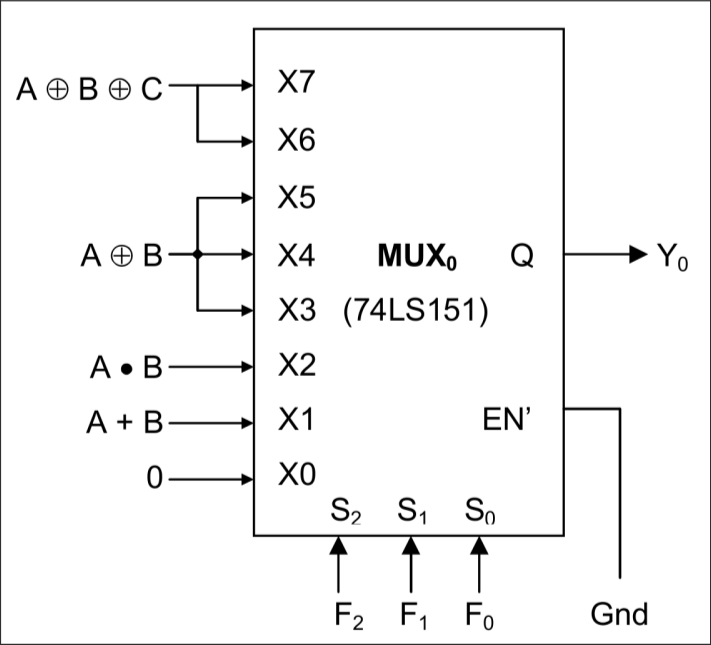
\includegraphics[width=0.34\textwidth]{circuit-y0.png}
            \caption{Circuit for $Y_0$}
        \end{figure}
    \end{itemize}
    \item \textbf{Design of $Y_1$:}
    \begin{itemize}
        \item The output $Y_1$ is only required for four operations corresponding to $F_2 = 1$.
        \item Hence, $F_2$ can be used as enable for the 8:1 MUX with selection being performed by $F_1 F_0 C$.
        \item Two consecutive data inputs of the MUX are assigned to each of the four operations -- corresponding to $C=0$ and $C=1$.
        \item For half-adder and half-subtactor operations, $C$ isn't an input. Therefore, the two data inputs corresponding to each of these operations are made identical.
        \item For full-adder and full-subtactor operations, $C$ affects the result. The Boolean expressions for carry and borrow were simplified for both $C=0$ and $C=1$ (for both operations), and the resulting expressions were connected to corresponding data inputs of the MUX.
        \item The resulting circuit for $Y_1$ is:
        \begin{figure}[H]
            \centering
            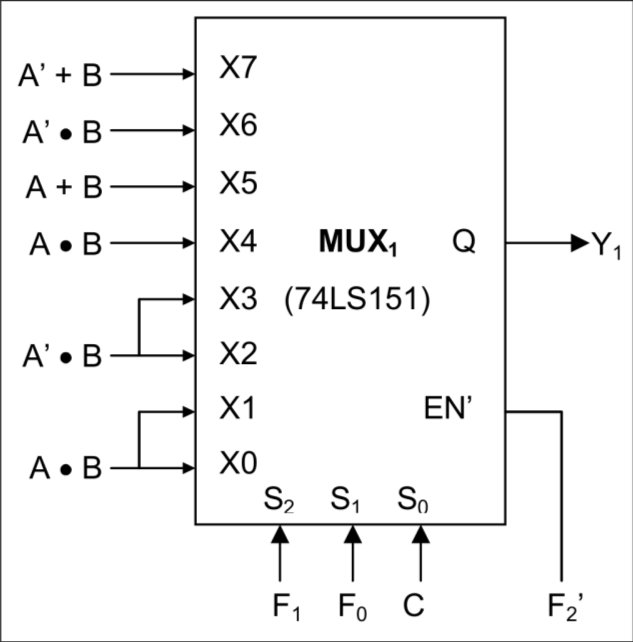
\includegraphics[width=0.34\textwidth]{circuit-y1.png}
            \caption{Circuit for $Y_1$}
        \end{figure}
    \end{itemize}
    \item \textbf{Generation of intermediate signals:} In the above discussion, we require 6 distinct Boolean fuctions. They can be generated as folows:
    \begin{itemize}
        \item $A+B$, $A \cdot B$, $\overline{A} \cdot B$ and $\overline{A} + B$ can be generated using 2:1 MUXes as follows:
        \begin{figure}[H]
            \centering
            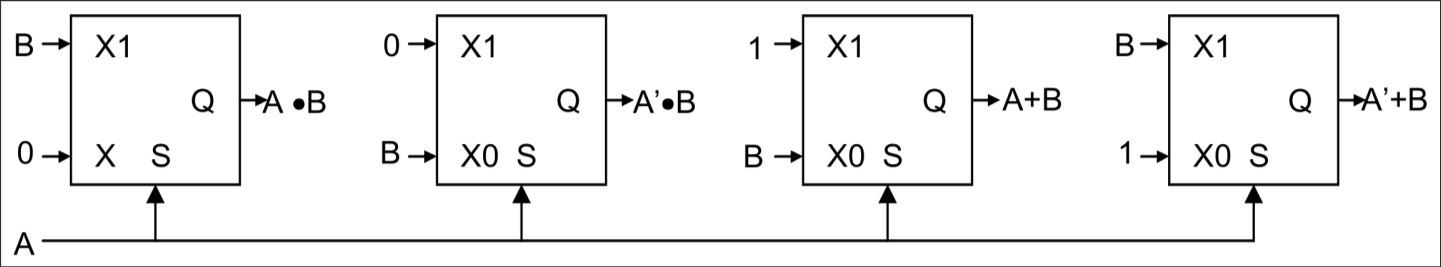
\includegraphics[width=0.8\textwidth]{circuit-intermediate.png}
            \caption{Circuit for Generating Intermediate Values using 2:1 MUXes}
        \end{figure}
        \item $A \oplus B$ and $A \oplus B \oplus C$ can be generated using and XOR gate (obviously).
    \end{itemize}
\end{enumerate}

\subsection{Implementation and Observation}
\begin{itemize}
    \item Place the required ICs on the breadboard and verify the operation of the quad 2-input XOR, quad 2:1 MUX, and the two 8:1 MUX ICs.
    \item Wire the circuit according to the designed circuit.
    \item Record the observed outputs in separate observation tables for all combinations of inputs for each ALU function (selected by function-select inputs).
\end{itemize}

\section{Observations}

\begin{minipage}[t]{0.48\textwidth}
\begin{table}[H]
    \centering
    \caption{$F_2 F_1 F_0 = 000$}
    \begin{tabular}{|ccc|cc|}
        \hline
        $A$ & $B$ & $C$ & $Y_1$ & $Y_0$ \\
        \hline
        X & X & X & - & 0 \\
        \hline
    \end{tabular}
\end{table}
\end{minipage}
\hfill
\begin{minipage}[t]{0.48\textwidth}
\begin{table}[H]
    \centering
    \caption{$F_2 F_1 F_0 = 001$}
    \begin{tabular}{|ccc|cc|}
        \hline
        $A$ & $B$ & $C$ & $Y_1$ & $Y_0$ \\
        \hline
        0 & 0 & X & - & 0 \\
        \hline
        0 & 1 & X & - & 1 \\
        \hline
        1 & 0 & X & - & 1 \\
        \hline
        1 & 1 & X & - & 1 \\
        \hline
    \end{tabular}
\end{table}
\end{minipage}

\medskip

\begin{minipage}[t]{0.48\textwidth}
\begin{table}[H]
    \centering
    \caption{$F_2 F_1 F_0 = 010$}
    \begin{tabular}{|ccc|cc|}
        \hline
        $A$ & $B$ & $C$ & $Y_1$ & $Y_0$ \\
        \hline
        0 & 0 & X & - & 0 \\
        \hline
        0 & 1 & X & - & 0 \\
        \hline
        1 & 0 & X & - & 0 \\
        \hline
        1 & 1 & X & - & 1 \\
        \hline
    \end{tabular}
\end{table}
\end{minipage}
\hfill
\begin{minipage}[t]{0.48\textwidth}
    \begin{table}[H]
    \centering
    \caption{$F_2 F_1 F_0 = 011$}
    \begin{tabular}{|ccc|cc|}
        \hline
        $A$ & $B$ & $C$ & $Y_1$ & $Y_0$ \\
        \hline
        0 & 0 & X & - & 0 \\
        \hline
        0 & 1 & X & - & 1 \\
        \hline
        1 & 0 & X & - & 1 \\
        \hline
        1 & 1 & X & - & 0 \\
        \hline
    \end{tabular}
\end{table}
\end{minipage}

\medskip

\begin{minipage}[t]{0.48\textwidth}
\begin{table}[H]
    \centering
    \caption{$F_2 F_1 F_0 = 100$}
    \begin{tabular}{|ccc|cc|} % 5
        \hline
        $A$ & $B$ & $C$ & $Y_1$ & $Y_0$ \\
        \hline
        0 & 0 & X & 0 & 0 \\
        \hline
        0 & 1 & X & 0 & 1 \\
        \hline
        1 & 0 & X & 0 & 1 \\
        \hline
        1 & 1 & X & 1 & 0 \\
        \hline
    \end{tabular}
\end{table}
\end{minipage}
\hfill
\begin{minipage}[t]{0.48\textwidth}
\begin{table}[H]
    \centering
    \caption{$F_2 F_1 F_0 = 101$}
    \begin{tabular}{|ccc|cc|} % 5
        \hline
        $A$ & $B$ & $C$ & $Y_1$ & $Y_0$ \\
        \hline
        0 & 0 & X & 0 & 0 \\
        \hline
        0 & 1 & X & 1 & 1 \\
        \hline
        1 & 0 & X & 0 & 1 \\
        \hline
        1 & 1 & X & 0 & 0 \\
        \hline
    \end{tabular}
\end{table}
\end{minipage}

\medskip

\begin{minipage}[t]{0.48\textwidth}
\begin{table}[H]
    \centering
    \caption{$F_2 F_1 F_0 = 110$}
    \begin{tabular}{|ccc|cc|}
        \hline
        $A$ & $B$ & $C$ & $Y_1$ & $Y_0$ \\
        \hline
        0 & 0 & 0 & 0 & 0 \\
        \hline
        0 & 0 & 1 & 0 & 1 \\
        \hline
        0 & 1 & 0 & 0 & 1 \\
        \hline
        0 & 1 & 1 & 1 & 0 \\
        \hline
        1 & 0 & 0 & 0 & 1 \\
        \hline
        1 & 0 & 1 & 1 & 0 \\
        \hline
        1 & 1 & 0 & 1 & 0 \\
        \hline
        1 & 1 & 1 & 1 & 1 \\
        \hline
    \end{tabular}
\end{table}
\end{minipage}
\hfill
\begin{minipage}[t]{0.48\textwidth}
\begin{table}[H]
    \centering
    \caption{$F_2 F_1 F_0 = 111$}
    \begin{tabular}{|ccc|cc|}
        \hline
        $A$ & $B$ & $C$ & $Y_1$ & $Y_0$ \\
        \hline
        0 & 0 & 0 & 0 & 0 \\
        \hline
        0 & 0 & 1 & 1 & 1 \\
        \hline
        0 & 1 & 0 & 1 & 1 \\
        \hline
        0 & 1 & 1 & 1 & 0 \\
        \hline
        1 & 0 & 0 & 0 & 1 \\
        \hline
        1 & 0 & 1 & 0 & 0 \\
        \hline
        1 & 1 & 0 & 0 & 0 \\
        \hline
        1 & 1 & 1 & 1 & 1 \\
        \hline
    \end{tabular}
\end{table}
\end{minipage}

\section{Tinkercad Simulation}
\noindent \textbf{Tinkercad Link:} \href{https://www.tinkercad.com/things/gCbjLD0KDY9-dsm-lab-4?sharecode=BRqWFJMTkXeqSe_WmEY9HMSCvb6GMnSRAZZ2AwisEFY}{\color{blue}Click here}
\begin{figure}[H]
\centering
    \centering
    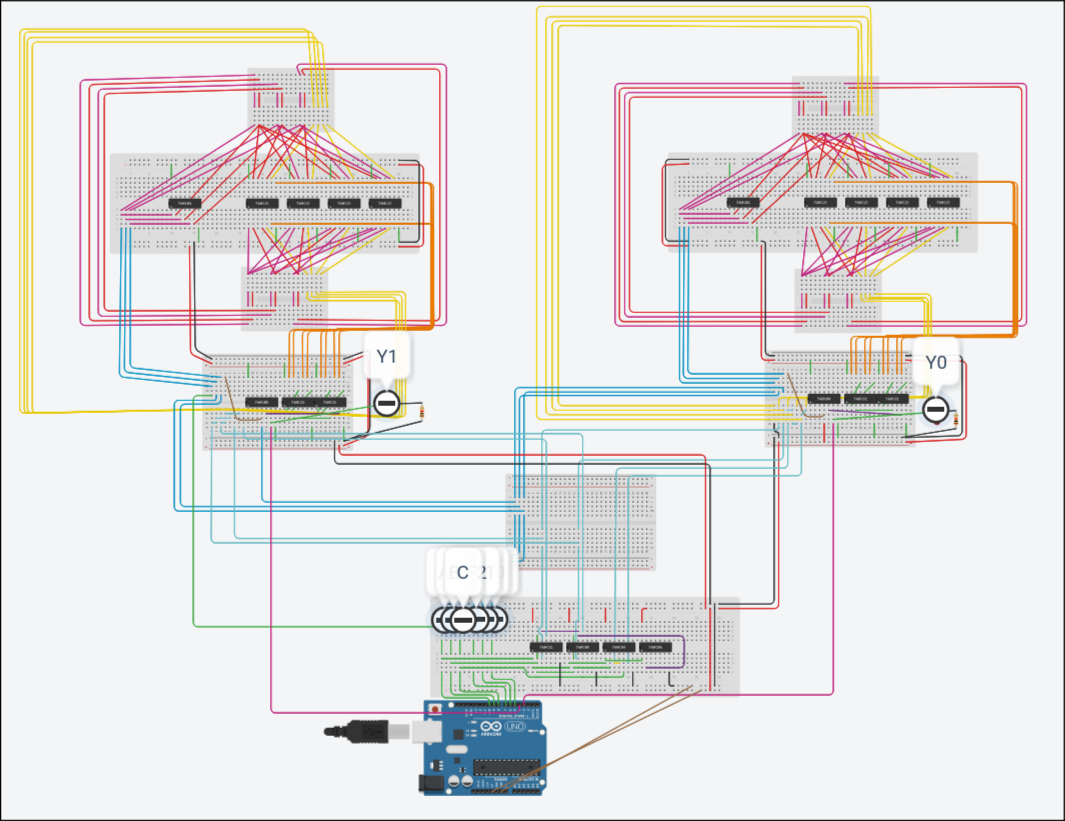
\includegraphics[width=\textwidth]{tc.png}
    \caption{Tinkercad Simulation Screenshot}
\end{figure}

\section{Hardware Setup Photograph}
\begin{figure}[H]
    \centering
    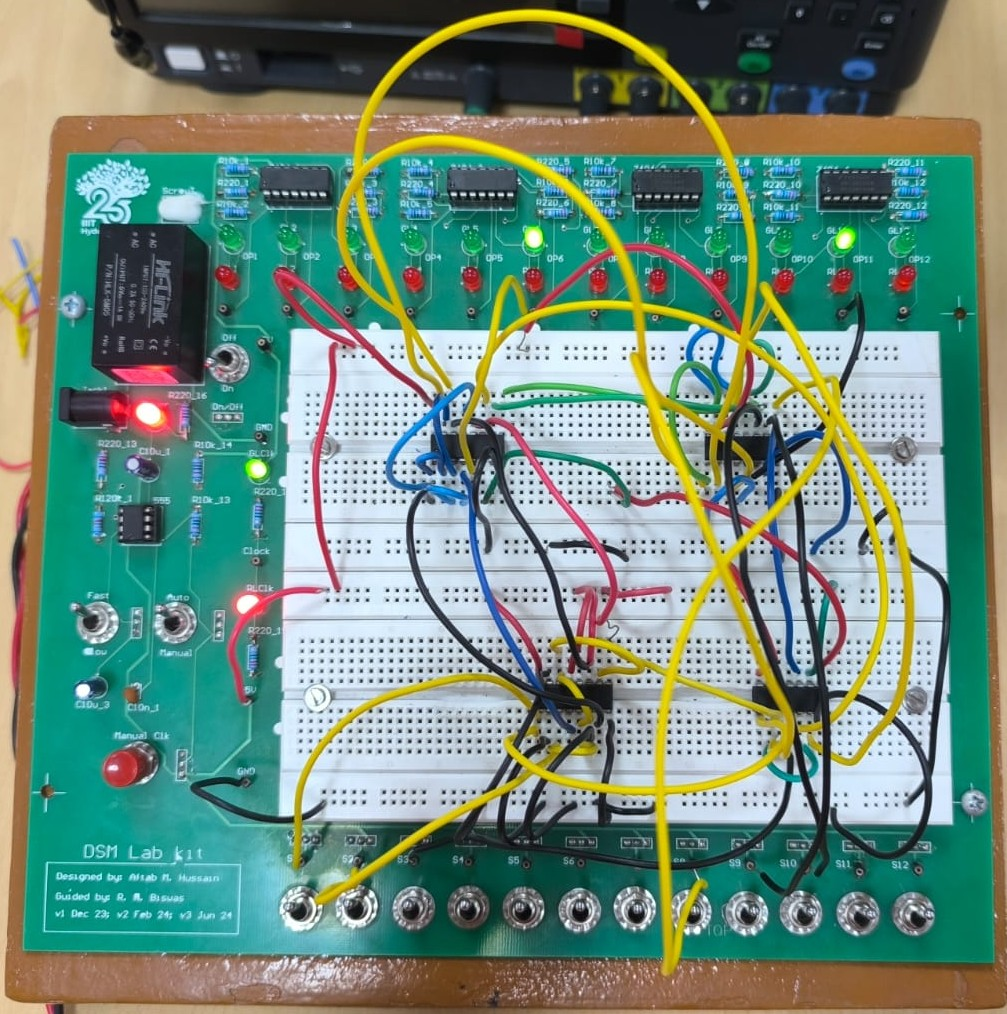
\includegraphics[width=0.8\textwidth]{lab.jpeg}
    \caption{Physical Circuit for Binary Half Adder}
\end{figure}

\section{Conclusion}
A 1-bit ALU was designed and implemented.

\end{document}